\documentclass[10pt,a4paper]{article}
\usepackage[margin=0.95cm]{geometry}
\usepackage[T1]{fontenc}
\usepackage{lmodern}
\usepackage{microtype}
\usepackage{graphicx}
\usepackage{booktabs}
\usepackage[colorlinks=true,urlcolor=blue]{hyperref}
\setlength{\parindent}{0pt}
\setlength{\parskip}{0pt}
\renewcommand{\arraystretch}{0.96}
\linespread{0.95}
\sloppy
\begin{document}
\begin{center}
\Large\textbf{Vote-distribution supervision for Galaxy Zoo morphology}\par
\vspace{-1pt}\normalsize\href{https://github.com/zhejunzhang529/galaxy-zoo-vote-supervision}{\textcolor{blue}{\underline{Code and saved results: GitHub}}}
\end{center}

\textbf{Research Background.} Galaxy morphology supports studies of galaxy evolution and structure. GZ2 collects multiple volunteer responses per image, so an argmax label discards disagreement. Disagreement may reflect observation limits, intermediate morphology or annotator differences; vote entropy alone is not causal evidence. Raw fractions are responses, not physical truth, and \textit{star or artifact} is the root screening class rather than a third galaxy morphology. The question is whether retaining votes improves probability fitting without obscuring the classification trade-off.

\textbf{Methodology.} The model is ImageNet-pretrained ResNet-18 with 128-pixel RGB input, Adam ($lr=3\times10^{-4}$, weight decay $10^{-4}$), batch size 32, and only layer4 plus the linear classifier unfrozen. Hard targets are one-hot argmax labels; soft targets are normalized raw vote fractions. The 128-pixel choice follows measured CPU throughput (65.72 versus 29.44 samples/s at 224 px). The soft-only search varied $lr\in\{10^{-4},3\times10^{-4}\}$, weight decay $\in\{0,10^{-4}\}$, and head-only versus layer4+head; validation soft CE selected the common configuration, with calibration discrepancy and earliest epoch as tie-breakers.

\begin{center}
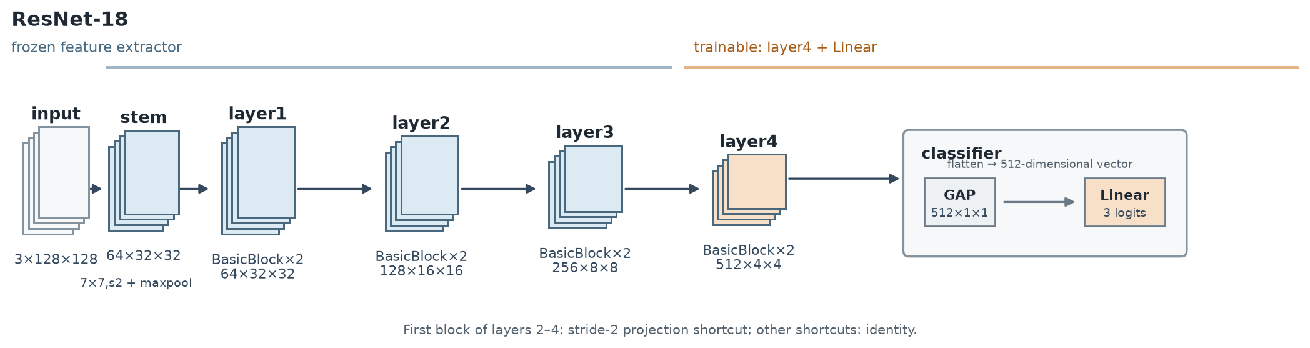
\includegraphics[width=0.90\linewidth]{round2_resnet/reports/assets/dis_resnet18_paper_architecture_report.pdf}
\par\vspace{-3pt}\scriptsize\textit{Figure 1. ResNet-18 feature-map schematic; GAP is flattened to a 512-dimensional vector before Linear produces 3 logits. The inset shows separate identity and projection shortcuts; BN/ReLU are omitted. Hard and soft runs share this architecture.}
\end{center}

\textbf{Results and Discussion.} Under the fixed-budget evaluation (three epochs; training sizes 3,100 and 10,000; fixed 750-object validation and a 10,000-object natural pool), the table reports means over three paired seeds. Mean-soft and hard-frequency baselines were $(CE,\,Brier,\,accuracy)=(0.7678,0.1676,0.7586)$ and $(0.8412,0.1819,0.7586)$.

\begin{center}\scriptsize\setlength{\tabcolsep}{5.5pt}
\begin{tabular}{lrrr}\toprule
training / target & CE & Brier & accuracy\\\midrule
3,100 hard & .8748 & .0880 & .8813\\
3,100 soft & .6156 & .0456 & .8908\\
10,000 hard & .8805 & .0851 & .8892\\
10,000 soft & .6053 & .0384 & .9034\\\bottomrule
\end{tabular}
\end{center}
The 10,000-object run also receives about 3.23 times as many updates while class-2 remains 34 training objects, so scale and update budget are confounded.

The separate 20-epoch train/validation diagnostic used the 3,100-object training split, fixed 750-object validation split and seed 20261119; it is not an independent evaluation:

\begin{center}
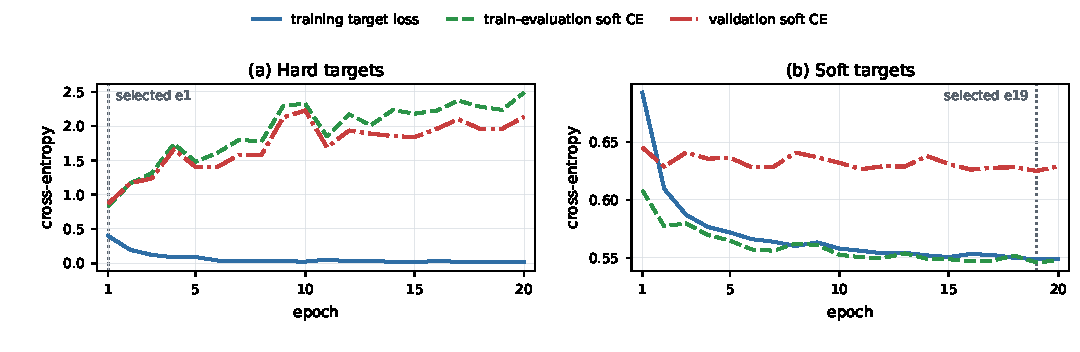
\includegraphics[width=0.82\linewidth]{round2_resnet/reports/assets/dis_training_curves_compact.pdf}
\par\vspace{-3pt}\scriptsize\textit{Figure 2. Blue is target loss: one-hot CE for hard and vote-distribution CE for soft; green/red are train-evaluation/validation soft CE. Dotted grey lines mark selected epochs (1 and 19); panels have independent y-scales.}
\end{center}

Hard training CE falls towards zero while validation soft CE rises from 0.8676 at epoch 1 to 2.1351 at epoch 20. Soft validation CE improves after epoch 3, reaching 0.6251 at epoch 19 and 0.6290 at epoch 20; the $10^{-4}$ soft run selected epoch 11 and ended at 0.6288. The separation is consistent with target mismatch and hard-target overfitting, but does not identify learning rate as the sole cause or prove convergence.

Finite learning-rate and regularisation checks found no consistent advantage for dropout 0.2 or weight decay $10^{-3}$. Selecting checkpoints by validation soft CE targets vote fit, rather than separate accuracy optimisation.

For the 10,000-object condition, the natural-pool group with $H>0.5462$ and $M\leq0.6897$ contained 4,520 objects ($H$: entropy of normalized votes; $M$: largest minus second-largest vote fraction). Soft/hard means were CE $0.794/1.136$, Brier $0.052/0.133$, and accuracy $0.808/0.793$: a conditional probability-fitting difference. On five \textit{star or artifact} objects, soft detected fewer at 3,100 but matched hard's mean at 10,000; repeated objects preclude population recall. GZ2 \texttt{extra} is an original-to-extra selection-shift test, not cross-survey OOD.

\begingroup\footnotesize
\textbf{References.} Willett et al. (2013), MNRAS 435, 2835; Walmsley et al. (2022), MNRAS 509, 3966; official GZ2 data: \url{https://data.galaxyzoo.org/}.
\endgroup
\end{document}
